\documentclass[border=6pt]{standalone}
\usepackage{tikz}
\usepackage[edges]{forest}
\usetikzlibrary{arrows.meta,positioning,calc,decorations.pathreplacing,shapes.geometric}
\begin{document}
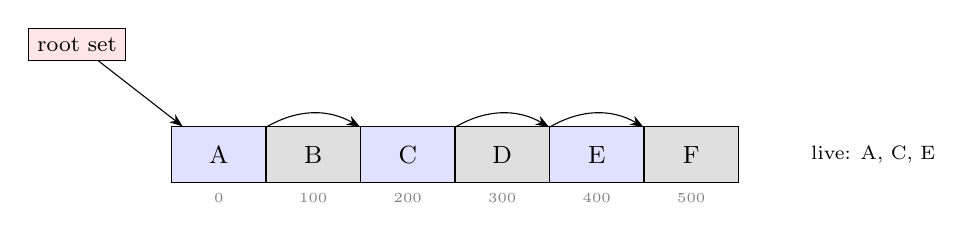
\begin{tikzpicture}[>=Stealth,font=\small]
\node[draw,minimum width=1.20cm,minimum height=0.7cm,fill=blue!12] (a) at (0.00,0.00) {A};
\node[draw,minimum width=1.20cm,minimum height=0.7cm,fill=gray!25] (b) at (1.20,0.00) {B};
\node[draw,minimum width=1.20cm,minimum height=0.7cm,fill=blue!12] (c) at (2.40,0.00) {C};
\node[draw,minimum width=1.20cm,minimum height=0.7cm,fill=gray!25] (d) at (3.60,0.00) {D};
\node[draw,minimum width=1.20cm,minimum height=0.7cm,fill=blue!12] (e) at (4.80,0.00) {E};
\node[draw,minimum width=1.20cm,minimum height=0.7cm,fill=gray!25] (f) at (6.00,0.00) {F};
\node[font=\tiny,gray,below=0.02cm of a] {0};
\node[font=\tiny,gray,below=0.02cm of b] {100};
\node[font=\tiny,gray,below=0.02cm of c] {200};
\node[font=\tiny,gray,below=0.02cm of d] {300};
\node[font=\tiny,gray,below=0.02cm of e] {400};
\node[font=\tiny,gray,below=0.02cm of f] {500};
\node[draw,fill=red!10,font=\footnotesize] (root) at (-1.8,1.4) {root set};
\draw[->] (root) -- (a);
\draw[->,bend left=30] (a) to (c); \draw[->,bend left=30] (c) to (e); \draw[->,bend left=30] (d) to (f);
\node[font=\scriptsize,anchor=west] at (7.4,0) {live: A, C, E};
\end{tikzpicture}
\end{document}
